%%%%%%%%%%%%%%%%%%%%%%%%%%%%%%%%%%%%%%%%%%%%%%%%%%%
%
%  New template code for TAMU Theses and Dissertations starting Fall 2016.
%
%
%  Author: Sean Zachary Roberson
%  Version 3.17.09
%  Last Updated: 9/21/2017
%
%%%%%%%%%%%%%%%%%%%%%%%%%%%%%%%%%%%%%%%%%%%%%%%%%%%
%%%%%%%%%%%%%%%%%%%%%%%%%%%%%%%%%%%%%%%%%%%%%%%%%%%%%%%%%%%%%%%%%%%%%%
%%                           TIME TO SOLUTION ESTIMATOR CHAPTER
%%%%%%%%%%%%%%%%%%%%%%%%%%%%%%%%%%%%%%%%%%%%%%%%%%%%%%%%%%%%%%%%%%%%%



\chapter{PARTITIONING OPTIMIZATION \label{cha:optimization}}
In Chapter \ref{cha:tts}, we have seen that we can estimate the time-to-solution for a sweep for different partitioning schemes.
We use the time-to-solution estimator as the objective function in two optimization methods.
The first optimization method utilizes scipy's optimize library, and the second method utilizes knowledge of a problem's mesh layout to assist in partition placement.
%%%%%%%%%%%%%%%%%%%%%%%%%%%%
\section{Scipy optimize}
The scipy optimize library \cite{scipy} provides many tools for optimizing an input function with local and global minimization techniques.
Our usage of the optimize library relies on the minimize function, using the basinhopping \cite{basinhoppingwales} method as the global optimizer, and the constrained Nelder-Mead method as the local optimizer.
We need a global optimization method for larger problem spaces to ensure that cut planes/lines are getting optimized over the entirety of the problem domain, rather than just moving the cut planes/lines close to our initial guess.

The black box tools of scipy optimize are too dependent on the smoothness of the function being optimized.
The time-to-solution estimator is not easily differentiable, and therefore not a smooth enough function even for the parameter spaces of a domain decomposed into 3 subsets in each dimension.
Although utilizing a tested and documented optimizer would have been ideal, it is clear that we need a method more uniquely suited for our problem.

\section{CDF Optimization}

The ``black box'' method using scipy optimize's basinhopping and constrained Nelder-Mead minimizers can function for very small parameter spaces.
However, even with modestly large parameter spaces such as the one seen in the Level 2 experiment (Fig. \ref{level2_nocut}), the time-to-solution estimator function is not smooth enough for scipy optimize to honor the constraints or bounds of the problem, leading to the time-to-solution estimator crashing.
This lead to the development of an alternative method, the CDF optimization method.

The CDF optimization method utilizes the geometrical information of the problem to attempt to find optimal cuts. This method prioritizes finding cut line locations that cut along a ``natural boundary'', and minimizing the total number of times the time-to-solution estimator needs to be run.
The time-to-solution estimator for moderately sized problems (such as the Level 2 experiment) can take up to 20 seconds to run for one set of partitions.
This rules out a brute force method of running every possible set of partitions.
Instead, we select our cut lines from the natural boundaries of the mesh.

A natural boundary is a subset boundary that coincides with the geometrical features of the mesh. In Fig.~\ref{natural_boundary_example}, we notice natural boundaries every centimeter in each dimension.
 \begin{figure}[h]
\centering
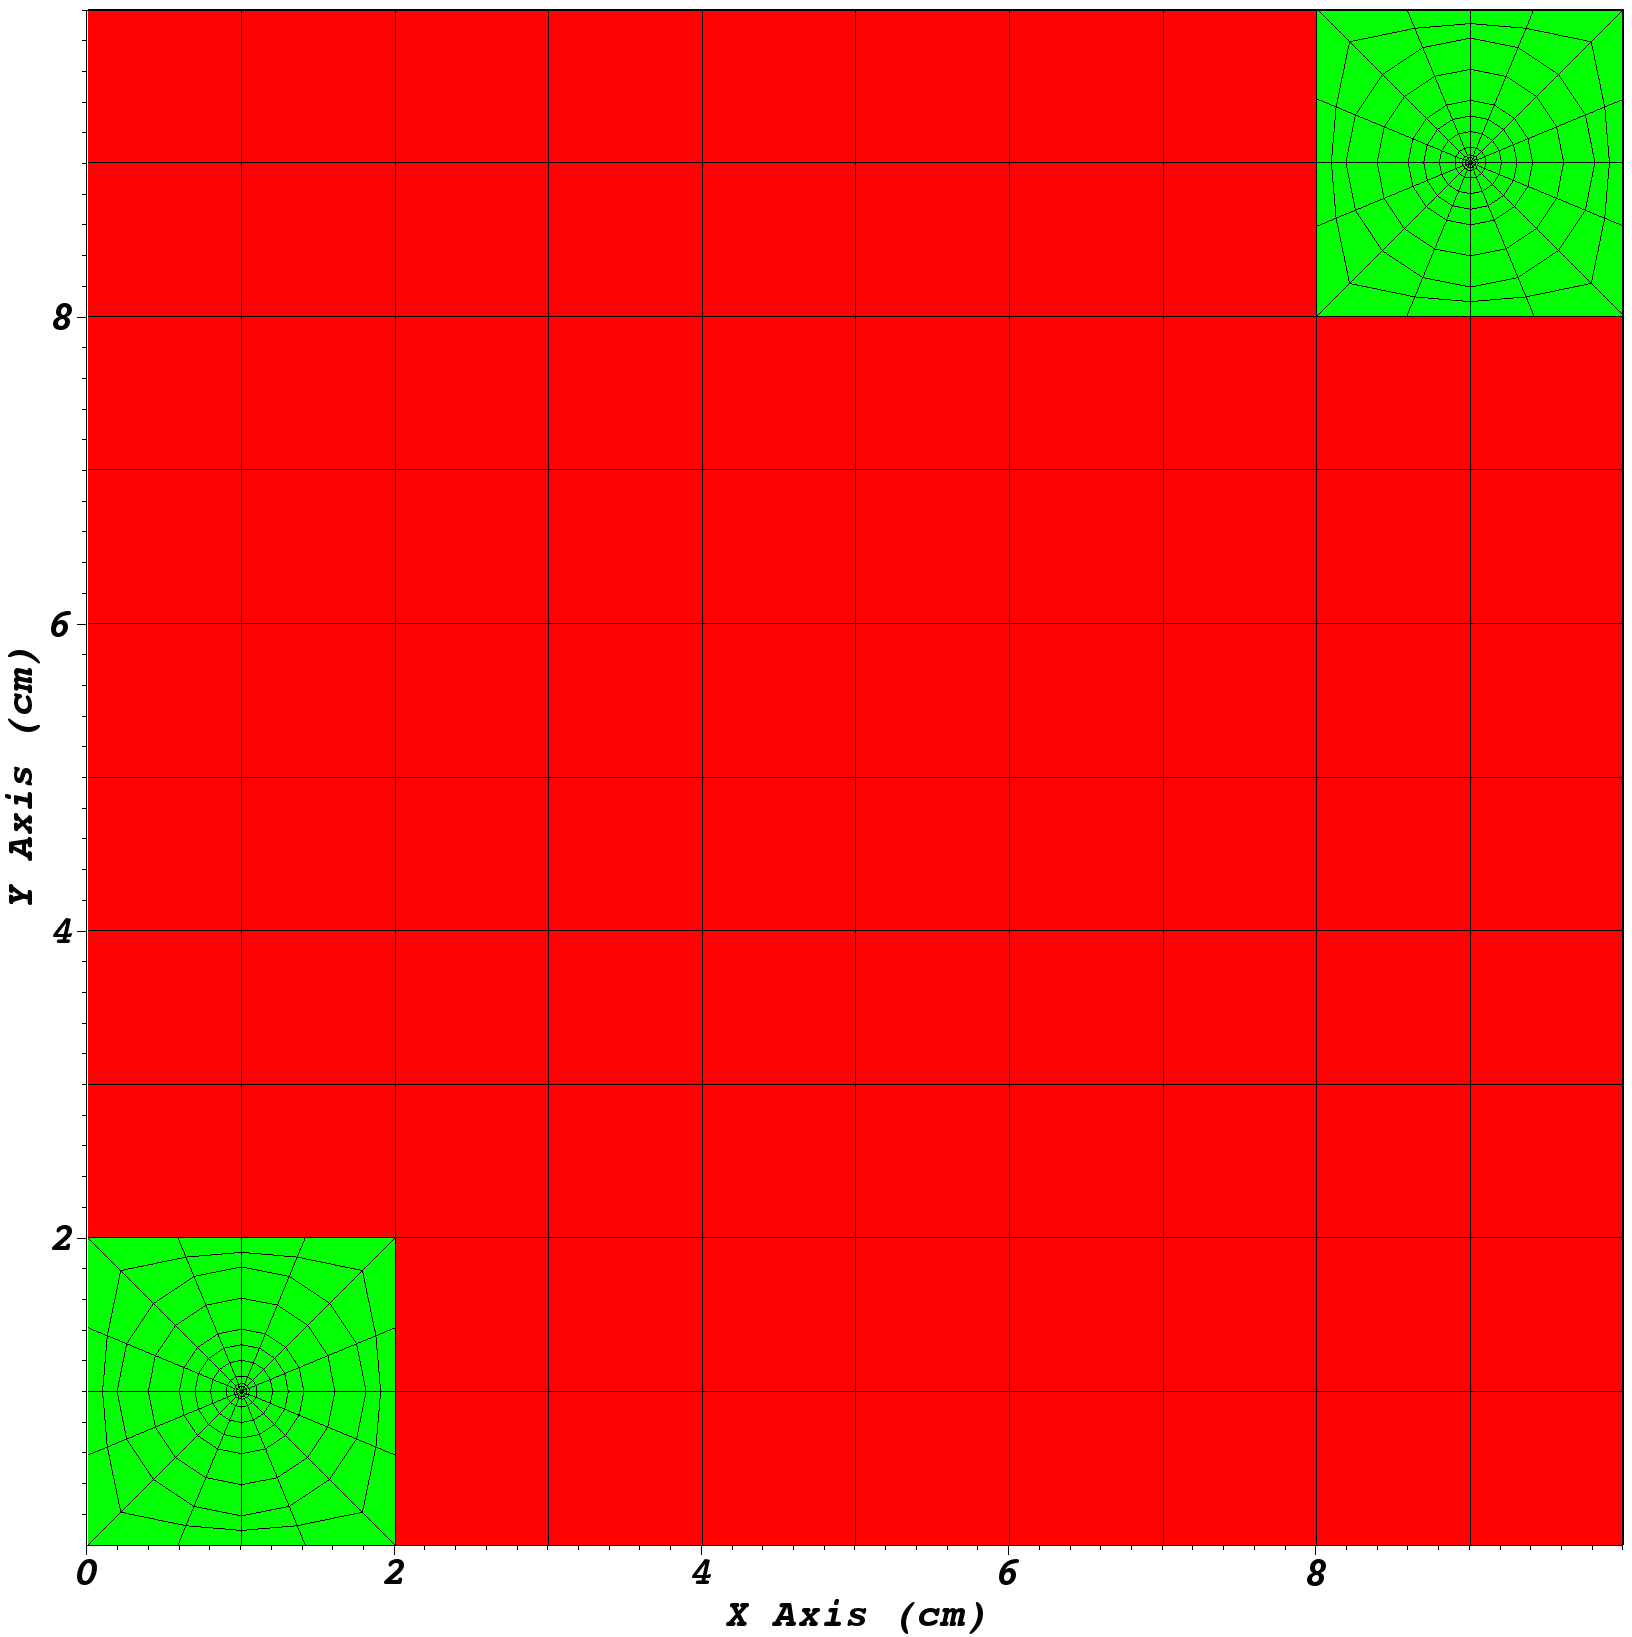
\includegraphics[scale=0.2]{../figures/spiderweb_10x10_sparse.png}
\caption{An unstructured mesh with natural boundaries at 1 cm intervals in both dimensions.}
\label{natural_boundary_example}
\end{figure}

The CDF optimization method will:
\begin{enumerate}
  \item Find the most suitable natural boundaries in the $x$ dimension,
  \item For each set of columns, find the most suitable natural boundaries in the $y$ dimension,
  \item Run all iterations of cut lines selected.
\end{enumerate}

\subsection{Finding Natural Boundaries}

In order to identify natural boundaries, we analyze the detailed cumulative distribution function (CDF) of the vertices in each dimension. The jumps in the CDF correspond to natural boundaries. Figure~\ref{vert_cdf} shows the x-vertex CDF of the mesh in Fig.~\ref{natural_boundary_example}.
\begin{figure}[h]
\centering
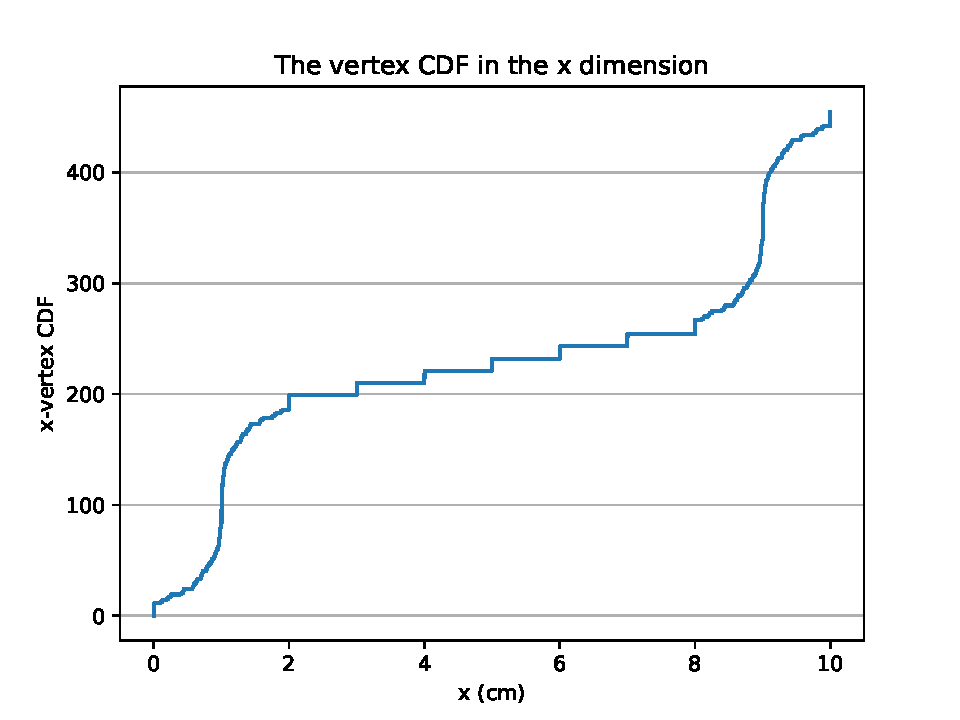
\includegraphics[scale=0.75]{../figures/xvertexcdf.pdf}
\caption{The x-vertex CDF of the mesh shown in Fig.~\ref{natural_boundary_example}}.
\label{vert_cdf}
\end{figure}

To identify where the jumps in the CDF occur, we take the derivative\jcr{I think your CDF's are functions of 1 variable only, so it's a derivative, no?} of the CDF and isolate the largest discontinuities in it. Figure~\ref{gradcdf} plots the derivative of the CDF shown in Fig.~\ref{vert_cdf}. \jcr{not sure I understand the jumps in the CDF derivative at the beginning and the end of the x axis. Why is it jumping? Numerical artifact? FROM TAREK: The global bounds of the problem are natural boundaries. In the unbalanced pin mesh, there are quite a few vertices along the global boundaries. }
\begin{figure}[h]
\centering
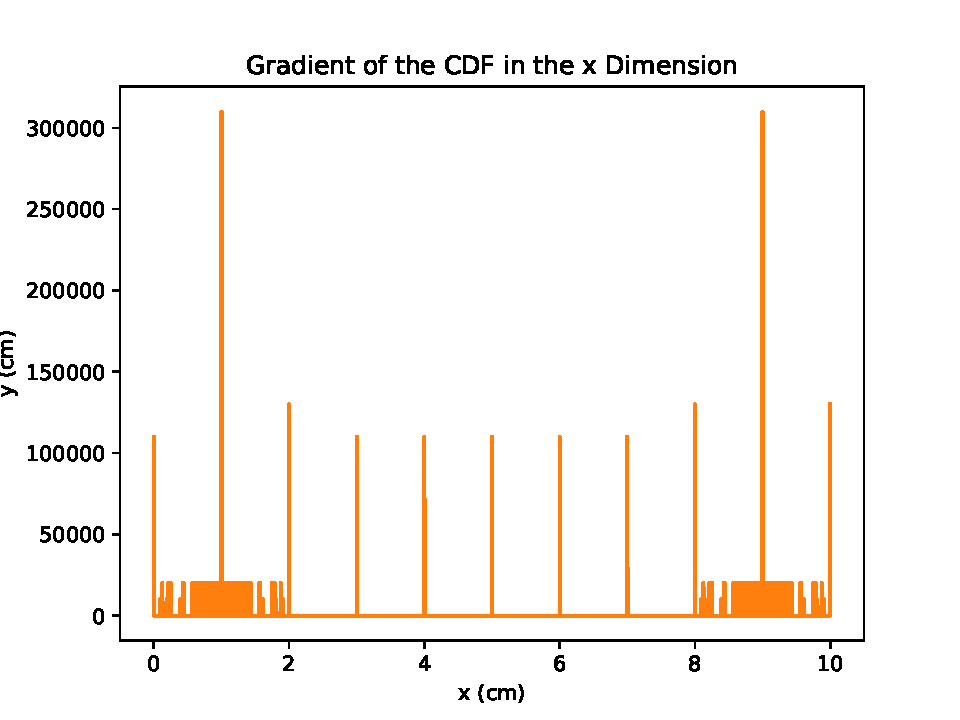
\includegraphics[scale=0.75]{../figures/gradcdf.pdf}
\caption{The derivative of the CDF shown in Fig.~\ref{vert_cdf}}.
\label{gradcdf}
\end{figure}
The largest discontinuities in Fig.~\ref{gradcdf} occur at the instances where there are natural boundaries all the way through the mesh, or at 1 cm intervals.

\FloatBarrier
\subsection{Finding Natural Boundaries for Sets of Columns}
In order to globalize the optimization of the cut lines per column, we set up a binary tree of test cases, such as the one shown in Fig.~\ref{binary_tree}. Each layer in the tree represents one set of $y$ cut lines. The first layer, or the root of the tree, represents the case where we try and find the natural boundaries in $y$ throughout all columns, in this case 4 columns. The next layer tries to find two sets of natural boundaries, one set of natural $y$ boundaries through the first two columns, and another set through the final 2 columns. Finally, the last case finds a set of natural $y$ boundaries in each individual column.

\begin{figure}[h]
\centering
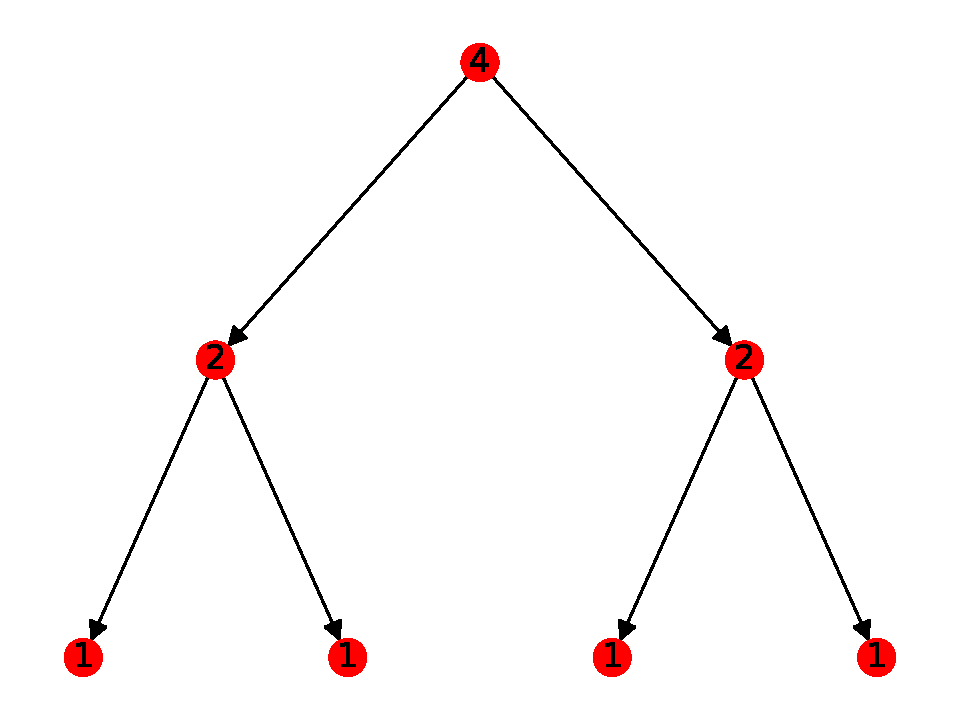
\includegraphics[scale=0.75]{../figures/binary_tree.pdf}
\caption{A binary tree where each node represents the number of columns we are attempting to find a natural boundary through.}
\label{binary_tree}
\end{figure}

Let's consider the mesh of the Level 2 experiment shown in Fig.~\ref{level2_nocut}.
We run this problem with 42 subsets in $x$ and 13 subsets in $y$.


\begin{figure}[h]
\centering
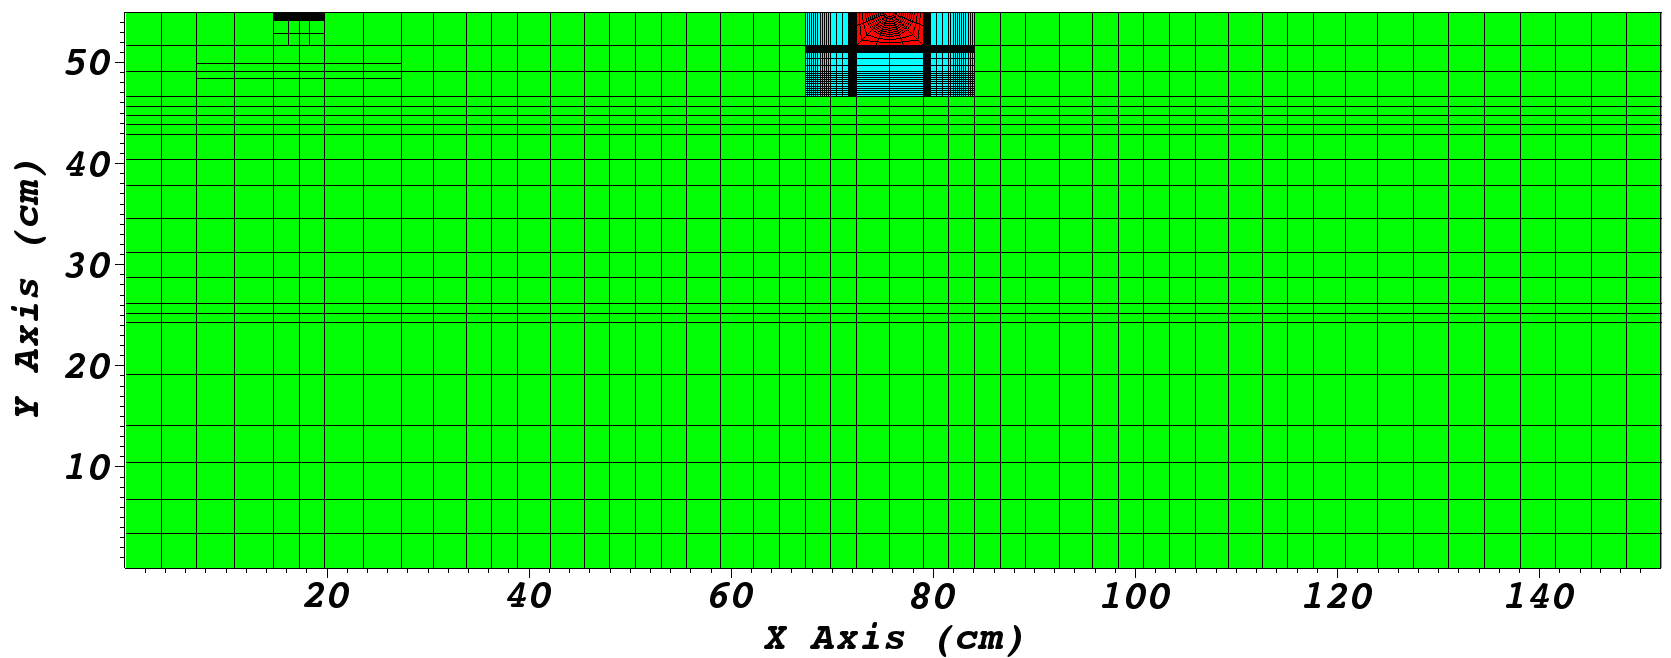
\includegraphics[scale=0.3]{../../figures/level2_nocut.png}
\caption{The mesh for the Level 2 experiment.}
\label{level2_nocut}
\end{figure}

\begin{figure}[h]
\centering
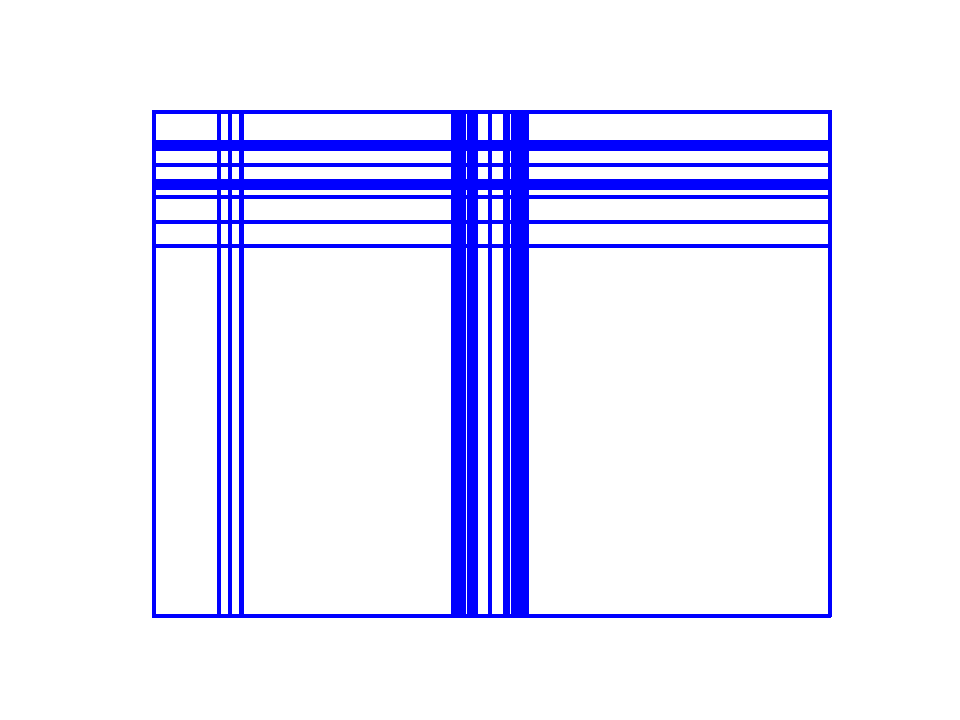
\includegraphics[scale=0.55]{../../figures/lvl2_suite_0.pdf}
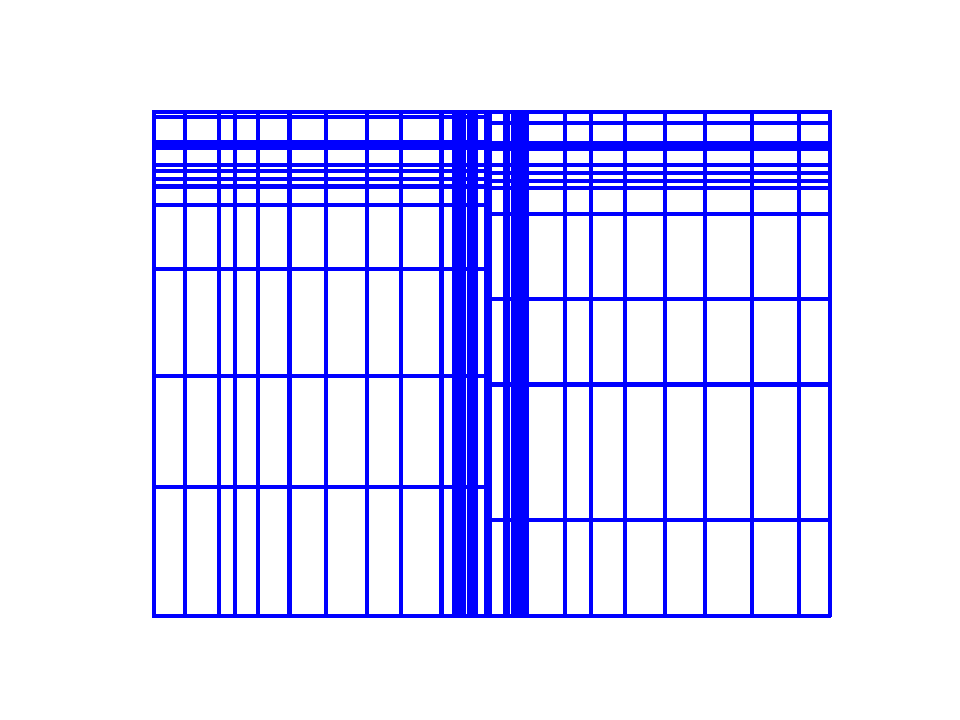
\includegraphics[scale=0.55]{../../figures/lvl2_suite_1.pdf}
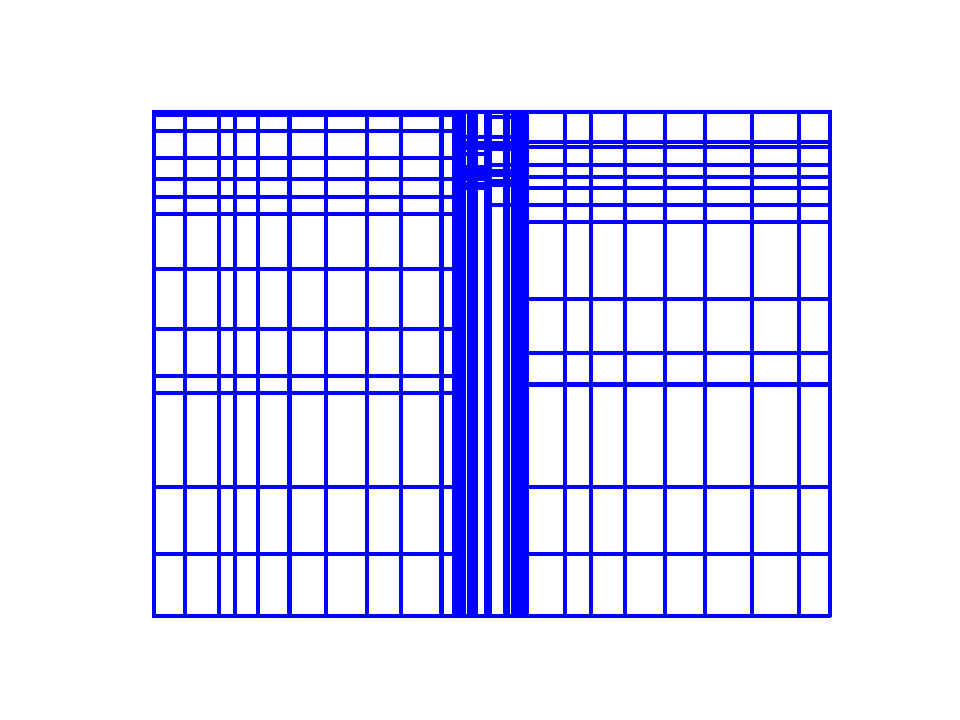
\includegraphics[scale=0.55]{../../figures/lvl2_suite_2.pdf}
\end{figure}

\FloatBarrier

\section{Optimization Results}
The CDF optimization method was run on the unbalanced pin mesh and the Level 2 experiment mesh.
The unbalanced pin mesh was run through the optimization suite from 2 to 10 subsets in each dimension.

